\documentclass{standalone}
\usepackage{tikz}
\usepackage{ctex,siunitx}
\setCJKmainfont{Noto Serif CJK SC}
\usepackage{tkz-euclide}
\usepackage{amsmath}
\usetikzlibrary{patterns, calc}
\usetikzlibrary {decorations.pathmorphing, decorations.pathreplacing, decorations.shapes,}
\begin{document}
\small
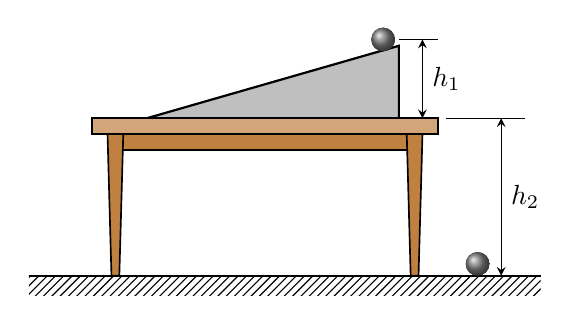
\begin{tikzpicture}[>=stealth,scale=1]
  \fill [pattern=north east lines](-3,-.25) rectangle (3.5,0);
  \draw [thick](-3,0)--(3.5,0);
  \draw [thick,fill=lightgray](-1.5,2) --(1.7,2.92)--(1.7,2);
  \draw [thin](1.7,3)--(2.2,3);
  \draw [thin](2.3,2)--(3.3,2);
  \draw [semithick,fill=brown!70](-2.2,1.8)rectangle(2.2,2);
  \draw [semithick,fill=brown](-1.9,1.8)rectangle(1.9,1.6);
  \draw [semithick,fill=brown](-2.0,1.8)--(-1.95,0)--(-1.85,0)--(-1.8,1.8)--cycle;
  \draw [semithick,fill=brown](2.0,1.8)--(1.95,0)--(1.85,0)--(1.8,1.8)--cycle;
  % \draw
  \fill [ball color=gray,semithick](2.7,0.15) circle (.15);
  \fill [ball color=gray,semithick](1.5,3.0) circle (.15);
  \draw [thin,<->](3.0,2)--(3.0,0)node[midway,right]{$h_2$};
  \draw [thin,<->](2.0,2)--(2.0,3)node[midway,right]{$h_1$};
  % \draw [densely dashed] (0,0.2) circle (.2);
\end{tikzpicture}
\end{document}